\section{Evaluation}
\label{lEvaluation}

In this chapter, the implementation of the migration procedure and the checkpointing routine are evaluated. The evaluation is split into different experiments, each of which consists of several test series. To assess the implementation's suitability in terms of the requirements stated in chapter \ref{lMethodology}, the experiments focus on different aspects of a common test-case. The first experiment (\acrshort{e}1) analyzes the downtime and overall migration time in the \textit{\acrshort{pe} live migration} under different networking conditions and state-sizes. The second experiment (\acrshort{e}2) addresses the \textit{\acrshort{pe} restoration}, focusing on the reprocessing performance. Lastly, checkpointing is examined by analyzing the impact of different state sizes on the checkpointing duration (\acrshort{e}3). Thereafter, the evaluation results and the proof of concept implementation are critically discussed in the light of the requirements. Finally, the consequential limitations of this thesis are briefly outlined.

\subsection{Setup}

\label{lEvaluationSetup}
\begin{figure}[!ht]
    \centering
    \graphicspath{{./figures/code/}}
    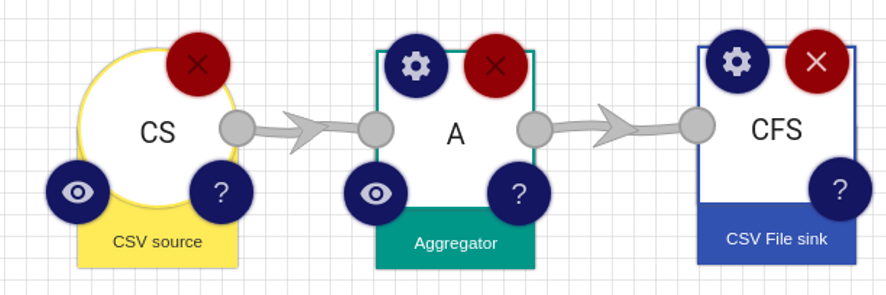
\includegraphics[width=\textwidth]{figures/visualizations/EvaluationPipelineSceenshot_1500.png}
    \caption{Screenshot of the test pipeline used throughout the evaluation}
    \label{fEvaluationPipeline}
\end{figure}

The test case used for the evaluation is the aforementioned \ref{cAggregation}. The needed \gls{pe}s were implemented in StreamPipes, and the pipeline was recreated, as shown in Figure \ref{fEvaluationPipeline}. Using \ref{cAggregation} as an illustrative case allows for a reliable way of determining whether the resulting output is consistent. The correct outcome is known since this pipeline is a composition of deterministic \gls{pe}s with a fixed input from a predefined \gls{csv} file. Any deviations from the expected output, which is also saved to a \gls{csv} file, flag inconsistent results.\par


\begin{figure}[!ht]
    \centering
    \graphicspath{{./figures/code/}}
    \includesvg[width=\textwidth]{figures/visualizations/EvaluationSetup_1500.svg}
    \caption{Setup for the evaluated experiments}
    \label{fEvaluationSetup}
\end{figure}


This test-case is evaluated on a setup of two devices, which are both connected to a local router via gigabit ethernet. The first device is a desktop PC with a 6-core, 3.60GHz AMD Ryzen 3600 processor with a total of 16GiB of RAM running Ubuntu 20.04. It simulates a centralized computing entity. A Raspberry Pi 4 single-board computer is deployed as the second device to simulate a small computing device in the fog. It is powered by a 4 core 1.50GHz ARM Cortex-A72 processor, has 4GiB of RAM, and runs a 64bit version of Raspberry Pi \gls{os} (a Debian based operating system optimized for the Raspberry Pi). For the evaluation of the test-case, the StreamPipes components are deployed, as depicted in Figure \ref{fEvaluationSetup}. The desktop PC hosts the micro-services mandatory for the StreamPipes deployment, namely Consul, Apache ActiveMQ, Apache Kafka, Apache ZooKeeper, InfluxDB, and Apache CouchDB, as well as the StreamPipes Backend and the user interface. These microservices are all deployed in independent but connected docker containers. Additionally to this base setup, the desktop PC hosts the source and sink \gls{pe}, as well as an instance of the aggregating \gls{pe}. The Raspberry Pi also hosts a containerized instance of the aggregating \gls{pe}.

\subsection{Results}
\label{lEvaluationResults}

Experiments \acrshort{e}1, \acrshort{e}2, and \acrshort{e}3 were conducted using the above-described test case on the test setup. The results of these experiments are presented in this sub-chapter.



\subsubsection{Pipeline Element Live Migration}
\label{lResultsOperatorStateMigration}

In the first experiment, the test case pipeline was set up using a source and sink \gls{pe} on the desktop PC and an aggregator \gls{pe} on the Raspberry Pi. Following a random wait time after starting the pipeline, the aggregator on the Raspberry Pi was migrated to the desktop PC using the \textit{\acrshort{pe} live migration}.\\
To simulate a real-world use case, this experiment was conducted while varying the network conditions and the state-size. The network conditions were varied to mimic the varying latencies encountered in fog computing \cite{Puliafito.2018}. This variation was realized by using the linux traffic control tools to add a network delay to traffic between the Raspberry Pi and the desktop PC. Three scenarios were distinguished. Tests with no added network delay (n0) (averaging a latency of 0.2ms between the devices), tests with an added network delay that is normally distributed averaging 100ms with a variance of 10ms (n100), and the last tests with a normally distributed network delay averaging 500ms with a variance of 50ms (n500), were conducted. State-sizes are the second varied factor. The variation of the state-size simulates different \gls{pe}s, whose states can have vastly different sizes. State-sizes range from sub-Kibibyte sizes, for example, in the aggregator used in the experiments, when it is configured to aggregate over a narrow window of past events, to state-sizes in the tens of \gls{mib}. For instance, a \gls{pe} that uses a machine learning model that changes over time due to reinforcement learning could have a larger state-size. The same aggregating \gls{pe} is used throughout all experiments and was therefore equipped with the capability to increase its state-size artificially. The state-size is increased by adding a String value with configurable length to the state. The experiment was conducted with three state-size setups. The first test-series was conducted with no added state (s0), the second one with 1\gls{mib} of added state (s1), and the last test-series with 5\gls{mib} of added state (s5).\par

In total, nine test-series were conducted, with differing network conditions and state-sizes between test-series. In all test-runs, the aggregating \gls{pe} was configured to aggregate the last ten values. The events were fed into the pipeline with an average frequency of one event every 300ms. Each test was performed ten times to achieve more reliable results.\par

\begin{figure}[!ht]
    \centering
    \subfloat[\centering Added average network delay of 0ms (n0)]{{\includesvg[width=5cm]{figures/statistics/OSMNetwork0_500.svg}}{\label{rOperatorStateMigrationNW0}}}%
    \subfloat[\centering Added average network delay of 100ms (n100)]{{\includesvg[width=5cm]{figures/statistics/OSMNetwork100_500.svg}}{\label{rOperatorStateMigrationNW100}}}%
    \subfloat[\centering Added average network delay of 500ms (n500)]{{\includesvg[width=5cm]{figures/statistics/OSMNetwork500_500.svg}}{\label{rOperatorStateMigrationNW500}}}%
    \captionsetup[subfloat]{labelformat=empty}
    \subfloat[\centering]{{\includesvg[width=15cm]{figures/statistics/OSMLegend_1500.svg}}}%
    
    \caption{Results of E1 under different networking conditions}%
    \label{rStateMigrationDuration}%
\end{figure}



Figure \ref{rStateMigrationDuration} depicts the total migration times for the different test-series. The total time is further broken down into 4 phases, corresponding to the migration procedure. In the first phase, the \gls{pe} is paused on the origin node. The current state is fetched from the \gls{pe} on the origin node in the second phase. In the third phase, the \gls{pe} is invoked on the target node with the previously fetched state. The migration is finalized by discarding the \gls{pe} on the origin node and saving the changed pipeline description. Since the \gls{pe} on the target node begins processing after its invocation, the sum of the first three phases provides an upper limit for the \gls{pe} downtime. The error bars in Figure \ref{rStateMigrationDuration} represent the standard deviation for the total time of migration.\\ 
In the test-series without added network delay (Figure \ref{rOperatorStateMigrationNW0}), the \gls{pe} downtime increased from 48ms with s0 to 112ms with s1 and further to 308ms with s5. In the test-series with an average of 100ms added network delay (Figure \ref{rOperatorStateMigrationNW100}), the \gls{pe} downtime rose from an average of 243ms with s0 to 911ms with s1 and 1278ms with s5. In the final test-series, with an average of 500ms added network delay (Figure \ref{rOperatorStateMigrationNW500}), the results increased similarly. They went from 1057ms with s0 to 2571ms at s1 and 3823ms at s5.\\
Overall, the results show two correlations. Firstly, the total time of migration and the \gls{pe} downtime both increase with an increasing state-size. Secondly, the total time of migration and the \gls{pe} downtime also increase with an increasing network delay. The phases whose duration increased the most with increasing state-size were phases 2 and 3. Across all network delays, the average duration of phase 2 rose by 540\% between tests with s0 and s1 and by 200\% between tests with s1 and s5. The average duration of phase 3 across all network delays increased by 150\% between tests with s0 and s1, and by 220\% between tests with s1 and s5. In contrast to these two phases, which involve handling the operator state, the duration of phases 1 and 4 did not change significantly in regards to the state-size. However, the duration of these two phases, together with phase 2 did rise with increasing network delay. The average duration of Phase 1 across all state-sizes rose by 1160\% between tests with n0 and n100, and by 490\% between tests with n100 and n500. A similar increase can be observed for phase 2, with an increase in duration by 880\% between tests with n0 and n100, and by 350\% between tests with n100 and n500. This relation can also be seen for phase 4, whose duration increases by 230\% between tests with n0 and n100, and by 360\% between tests with n100 and n500.\par

\begin{figure}[!ht]
    \centering
    \subfloat[\centering CPU load in an illustrative test case]{{\includesvg[width=7.5cm]{figures/statistics/OperatorStateMigrationCPUSingleCase_750.svg}}{\label{rOperatorStateMigrationCPUSingle}}}%
    \subfloat[\centering Average CPU load during \textit{\acrshort{pe} live migration}]{{\includesvg[width=7.5cm]{figures/statistics/OperatorStateMigrationCPUAverage_750.svg}}{\label{rOperatorStateMigrationCPUAverage}}}%
    \caption{CPU load in the \gls{pe}'s container on the Raspberry Pi}%
    \label{rOperatorStateMigrationCPU}%
\end{figure}


In addition to these measurements, the \gls{cpu} on the Raspberry Pi was monitored. Figure \ref{rOperatorStateMigrationCPUSingle} shows an illustrative test run with s5 and n0. The \gls{cpu} load is on a level of under 10\% for most of the time with three spikes of 40\% to 60\% at 2.4 seconds, 5.4 seconds, and 7.2 seconds. The first two spikes correspond with the timing of the checkpointing. The last spike coincides with the migration.\\
To further inspect the \gls{cpu} load during the migration, a follow-up test-series was conducted, for which the artificial state-size was increased to 50\gls{mib}. Figure \ref{rOperatorStateMigrationCPUAverage} shows the average \gls{cpu} load for the migration timeframe. During this timeframe, an increase in the \gls{cpu} load to 50\% was observed.\par

The last evaluated factor was the consistency of the results. The consistency was assessed by analyzing the output of the sink \gls{pe}. As previously explained, the expected output is deterministic. Therefore, the consistency check was conducted by comparing the sink output with the expected output. In a total of 110 evaluated runs, the result was always consistent. 
%This held true, even for an average time between events of xx and xx.

\subsubsection{Pipeline Element Restoration}
\label{lResultsOperatorStateRestoration}
For the second experiment, the test case pipeline was set up using a source, sink, and aggregator \gls{pe} on the desktop PE. After a random period of time, the aggregator on the desktop PC was discarded to simulate a \gls{pe} becoming interrupted. Thereafter, a random waiting period followed, after which the aggregator was restored on the Raspberry Pi using the \textit{\acrshort{pe} restoration}. Since checkpointing is done at regular intervals, the random timing of discarding the \gls{pe} leads to a variation in the number of events that need to be reprocessed. As the time period between discarding and restoring the \gls{pe} is also random, the number of intermediary events is also irregular. Intermediary events are the events occurring in the time between the interruption of the \gls{pe} and the start of the restoration (as described in section \ref{lMigrationConcept} Figure \ref{fTimingOSR}).\par

For this experiment, a total of 100 test runs were conducted. In all test-runs, the aggregating \gls{pe} was configured to aggregate the last ten values. The state-size was artificially increased by 1\gls{mib}. The events were fed into the pipeline with an average frequency of one event every 300ms. Additionally, the \gls{pe}-level checkpointing was configured to a frequency of checkpointing once every five seconds.\par


\begin{figure}[!ht]
    \centering
    \subfloat[\centering Duration of reprocessing in relation to the number of reprocessed events]{{\includesvg[width=7.5cm]{figures/statistics/StateRestorationScatterReprocess_750.svg}}{\label{rOperatorStateRestorationReprocessing}}}%
    \subfloat[\centering Duration of processing intermediate events in relation to the number of intermediately processed events]{{\includesvg[width=7.5cm]{figures/statistics/StateRestorationScatterIntermediate_750.svg}}{\label{rOperatorStateRestorationIntermediateProcessing}}}%
    \caption{Duration of reprocessing and intermediately processing events after \textit{\acrshort{pe} restoration}}%
    \label{rOperatorStateRestorationDuration}%
\end{figure}


Figure \ref{rOperatorStateRestorationDuration} displays the results of E2. In Figure \ref{rOperatorStateRestorationReprocessing}, the time spent reprocessing is depicted in dependence on the number of reprocessed events. The results show an increase in processing time with an increase in the number of reprocessed events. A similar relation can be observed between the time spent processing intermediary events and the number of intermediary processed events (Figure \ref{rOperatorStateRestorationIntermediateProcessing}). The average time per reprocessed event is 0.608ms, which is significantly lower than the average time per intermediary processed event, which takes 1.109ms on average. This difference can be attributed to the fact that the result of processing intermediary events is output by a Kafka producer, whereas the output of reprocessing is discarded.\par

\begin{figure}[!ht]
    \centering
    \graphicspath{{./figures/code/}}
    \includesvg[width=\textwidth]{figures/statistics/stateRestorationCPU_1500.svg}
    \caption{\gls{cpu} load in the \gls{pe}'s container on the Raspberry Pi for an illustrative test case}
    \label{rOperatorStateRestorationCPU}
\end{figure}

The \textit{\acrshort{pe} restoration} has a significant impact on the \gls{cpu} load. This is shown in Figure \ref{rOperatorStateRestorationCPU}, which depicts the \gls{cpu} load of the aggregating \gls{pe}'s container on the Raspberry Pi in a selected test-run. In the time between 0.338 seconds and 0.570 seconds, 191 events were reprocessed. After that, 309 intermediary events were processed until 1.120 seconds. Over this period, the \gls{cpu} load increased to around 90\%. Once regular event processing took over, the \gls{cpu} load dropped to under 10\%, where it leveled off.\par

To evaluate the consistency of the \textit{\acrshort{pe} restoration}, five additional test-runs were conducted. For these test runs, the setup was adjusted. Instead of initially deploying the test pipeline solely on the desktop PC, the aggregator was deployed on the Raspberry Pi. In the test-runs, the Raspberry Pi was forcefully interrupted by cutting off its power connection a random time period after the pipeline was started. Thereafter, a \textit{\acrshort{pe} restoration} with the desktop PC as target node was performed.\\
The resulting output of the five conducted test runs shows no inconsistencies.


\subsubsection{Checkpointing}
\label{lResultsCheckpointing}
The checkpointing performance was assessed based on the data gathered in E1. Figure \ref{rCheckpointingDuration} depicts the average time checkpointing the aggregator's operator state takes on the Raspberry Pi, depending on the additional state size. While the duration of checkpointing was only 3.1ms in the tests with no added state, the duration increased to 23.8ms at 1\gls{mib} of artificially added state and rose to 84.1ms with 5\gls{mib} of added state. The share of the serialization time in the total checkpointing duration also increased from 0.3\% with no added state to 32.3\% with 1\gls{mib} added state and further to 40.6\% with 5\gls{mib} added state. 

\begin{figure}[H]
    \centering
    \graphicspath{{./figures/code/}}
    \includesvg[width=11.1cm]{figures/statistics/CheckpointingTime_1110.svg}
    \caption{Checkpointing duration in relation to the operator state size}
    \label{rCheckpointingDuration}
\end{figure}


\subsection{Discussion}
\label{lDiscussion}

In this discussion, the implementation and the evaluation results are examined against the backdrop of the requirements. From thereon, the limitations of this thesis are derived.\par

\textbf{Basic Functionality}\par
The basic functionality required by the \ref{rBasicMigration} and the \ref{rRecovery} requirement is provided by the conceptual framework developed in \ref{lMigrationConcept}. The proof of concept implementation could satisfy these requirements throughout the experiments.\\
Therefore, the \ref{rBasicMigration} and the \ref{rRecovery} requirement are met.\par

\textbf{Problem Handling}\par
\ref{rProblemHandling} is another requirement concerning the migration functionality. While the \textit{\acrshort{pe} live migration} implementation addresses problem handling, the \textit{\acrshort{pe} restoration} does it only to a lesser extent. 
In the \textit{\acrshort{pe} live migration}, the \gls{pe} on the origin node is paused until the correct invocation on the target node is confirmed. Processing is restarted on the origin node if the \gls{pe} cannot be invoked on the target node, providing a safety measure for problems during the migration. The \textit{\acrshort{pe} restoration} implementation only informs about the restoration attempt's success or failure but does not provide any active measure to address problems.\\
Overall, the \ref{rProblemHandling} requirement is addressed partly by the conceptual framework. To fully meet this requirement, software components that orchestrate the migration (e.g., decide when and with which target to migrate) need to react to the feedback received from the migration procedures.\par


\textbf{Consistency}\par
Achieving an exactly-once semantic with a consistent output is the best-case scenario, according to the \ref{rConsistency} requirement. The \textit{\acrshort{pe} live migration} is implemented with the intention of an exactly-once semantic. The results of E1 showed no inconsistencies, providing evidence that the exactly-once semantic was achieved and that the operator state is migrated as desired.\\
The \textit{\acrshort{pe} restoration} implementation is designed to provide an at-least-once semantic, with the intention to avoid processing events a second time when possible. The preliminary results from E2 showed no inconsistencies, meaning that the correct operator state was reconstructed and that no event was not processed or processed twice (except for reprocessing, which does not output events).\\
Therefore, the consistency requirement was largely met. A possible further improvement of the \textit{\acrshort{pe} restoration} could be achieved with Apache Kafka as an intermediary message broker, using its in-build capabilities for exactly-once processing \cite{Narkhede.2017}. On the flip side, this would add additional overhead to event processing.\par

\textbf{\acrlong{pe} Downtime}\par
The \ref{rDowntime} requirement states that the \gls{pe} downtime should be as low as possible, which is addressed by the developed conceptual framework and the implementation. The evaluation results reveal factors that influence the \gls{pe} downtime in both the \textit{\acrshort{pe} live migration} and the \textit{\acrshort{pe} restoration}.\\
For the \textit{\acrshort{pe} live migration}, the results of E1 imply a positive correlation between state-size and migration duration (p=xx) and a positive correlation between network delay and migration duration. This increase in the migration duration also entails an increase in the \gls{pe} downtime.\\
In E2, the \textit{\acrshort{pe} restoration} was examined. A positive correlation between the number of reprocessed events and the reprocessing duration was observed (p<0.0001). A positive correlation was also found in the relation between the number of intermediate events processed and the duration of the intermediate processing of events (p<0.0001).\\
The information gathered in E1 reveals a potential for downtime improvement. A high \gls{pe} downtime can be attributed to network impairments and great state-sizes. In a situation where the origin node of the \gls{pe} that should be migrated suffers from a high network delay, it could be beneficial to restore the \gls{pe} on the target node from an old checkpoint using the \textit{\acrshort{pe} restoration} procedure (instead of \textit{\acrshort{pe} live migration}). The \textit{\acrshort{pe} restoration} is favorable if getting the checkpoint from the database and reprocessing events can be done faster than getting the \gls{pe}'s most recent state. However, the decision between the procedures additionally depends on the \gls{pe} in question since it can be suspected that different \gls{pe}s vary in their performance when reprocessing events. Thus, a holistic approach is needed to address this problem.\\
In conclusion, there is further potential to lower the \ref{rDowntime}, even though the \gls{pe} \ref{rDowntime} is considered in the proof of concept implementation. Using a holistic approach and applying the tactics proposed in related works could help to minimize the downtime.\par


\textbf{Development}\par
According to the \ref{rDevelopment} requirement, the migration capability should add as little effort as possible to the development of \gls{pe}s. This is addressed in the proof of concept implementation by providing the universal \textit{StateHandler}, which offers a convenient way for developers to expose the processing state. Additionally, the buffer and routing state are handled automatically.\\
Overall, the \ref{rDevelopment} requirement is predominantly met, only requiring a minor additional effort in the \gls{pe} development.\par


\textbf{Fog Compatibility}\par
The \ref{rFogCompatibility} requirement demands resource constraints and varying networking conditions in the fog to be addressed.\\
The influence of varying network conditions on the \textit{\acrshort{pe} live migration}, and all associated steps were examined in E1. The \textit{\acrshort{pe} live migration} was not susceptible to faults or inconsistencies with network delays between 0ms and 500ms. However, the network delay had a significant impact on the duration of the migration. By allowing workload mobility, the \gls{pe} migration gives the possibility to lower the latency by relocating \gls{pe}s to available nodes with lower latency.\\
The impact on \gls{cpu} load was investigated for \textit{\acrshort{pe} live migration} in E1 and for \textit{\acrshort{pe} restoration} in E2. The results in E1 showed an increased \gls{cpu} load of around 50\% during migration. In E2, the \gls{cpu} load was even higher during event reprocessing and intermediate processing, culminating at more than 90\%. These observations were made with a \gls{pe} deployed on a Raspberry Pi, simulating a fog node with limited computing capabilities. Even though the \gls{cpu} load increased during migration and checkpointing, these increases resembled short spikes that were limited to the duration of the respective action. During the tests, the Raspberry Pi's limited capabilities did not provoke faults in the migration procedure and did also not impact the result's consistency. Workload mobility enables \gls{pe} relocation based on resource constraints, which could allow a more balanced and effective resource usage across the devices deployed in the fog.\\
These preliminary results suggest that the developed proof of concept is deployable across devices with different computing capabilities and under varying networking conditions, meeting the \ref{rFogCompatibility} requirement.\par


All in all, the set requirements are predominantly met by the proof of concept implementation. Out of all requirements, the \ref{rProblemHandling} and the \ref{rDowntime} requirement show the most potential for further improvement.

\textbf{Limitations}\par

The limitations of this thesis can be categorized into the limitations of the developed conceptual framework, the limitations of the implementation, and the limitations of the evaluation.\par

A clear limitation of the developed conceptual framework is that it revolves around two distinct procedures, which address different cases. This is a limitation since it requires a preceding categorization of the current case to decide which procedure to choose.\\
Additionally, the conceptual framework is developed for a use case with a centralized orchestrator. The centralization in \gls{dlac} limits the possibility of decentralized fog computing because it creates a dependency on a centralized orchestrator and a centralized database to provide globally available checkpoints.\par

The implementation is limited by technology dependency, missing handling of interrupted \gls{pe}s, and compatibility constraints.\\
A dependency exists to Apache Kafka because the implementation relies on its integrated offset management to handle the buffer state. This technology dependency could be addressed by persisting the buffer state, or even the whole operator state to the upstream \gls{pe}, as proposed by Fernandez et al. \cite{CastroFernandez.2013}.\\
Additionally, the implementation lacks measures to handle interrupted \gls{pe}s. However, these measures are needed to guarantee that a supposedly interrupted \gls{pe} does not come back to life, meaning that it does not start processing events again. A \gls{pe} coming back to life is undesirable because it would most certainly introduce inconsistencies in the resulting output event stream. Therefore, it needs to be discarded in such a case. One scenario where this could happen is when a \gls{pe} is restored on a new node because of temporary networking problems on its origin node. If the \gls{pe} on the origin node reconnects to the network, it might start processing events again.\\
Furthermore, the proof of concept implementation cannot be deployed on devices with a 32-bit arm processor. This is due to RocksDB, which only supports arm processors with a 64-bit architecture that supports the "AArch64" instruction set. This can be problematic since small computing devices used as fog nodes might have an insufficient arm processor.\par

Due to the high number of possibly influencing variables on the implementation's performance, only a selection of them could be examined in the evaluation.\\
Neither E1, nor E2 addresses other components of varying networking conditions than latency. For example, packet loss could also be problematic in the context of fog computing.\\
Another apparent weakness of the evaluation is that only experiments in a single test scenario and with a single \gls{pe} were conducted. This neglects the differences between \gls{pe}s, ranging from the complexity of the processing state to the effort needed to process events. These factors can be expected to influence the invocation time from an old state, as well as the reprocessing duration.\\
Lastly, the evaluation was conducted in a highly controlled environment. To determine the real-world performance, more realistic test scenarios need to be explored, for example, \ref{cMedical}.\par
